\section{Measuring Possible Surveillance Opportunities}
\label{measure}

\subsection{Methodology}

\begin{enumerate}
\item Curl the domain.
\item Extract third party domains from the curled domain.
\item Locally resolve each domain (and third party domains).
\item Consolidate DNS responses into a set of /24 subnets.
\item Traceroute to each /24.
\item Map traceroutes to country-level paths.
\end{enumerate}

\subsection{Results}

\begin{figure}
\centering
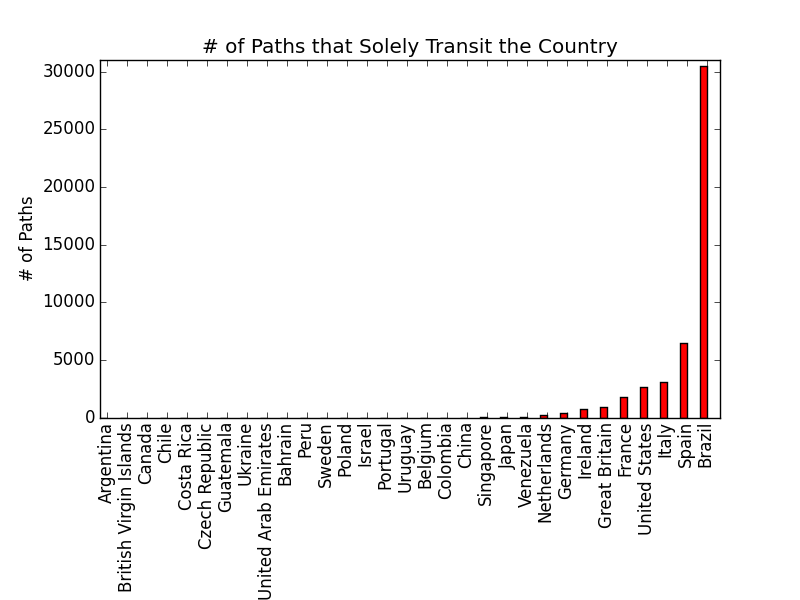
\includegraphics[width=.5\textwidth]{transit_graph}
\caption{The number of paths that solely transit a country (do not end in the country).}
\label{fig:transit}
\end{figure}

\begin{figure}
\centering
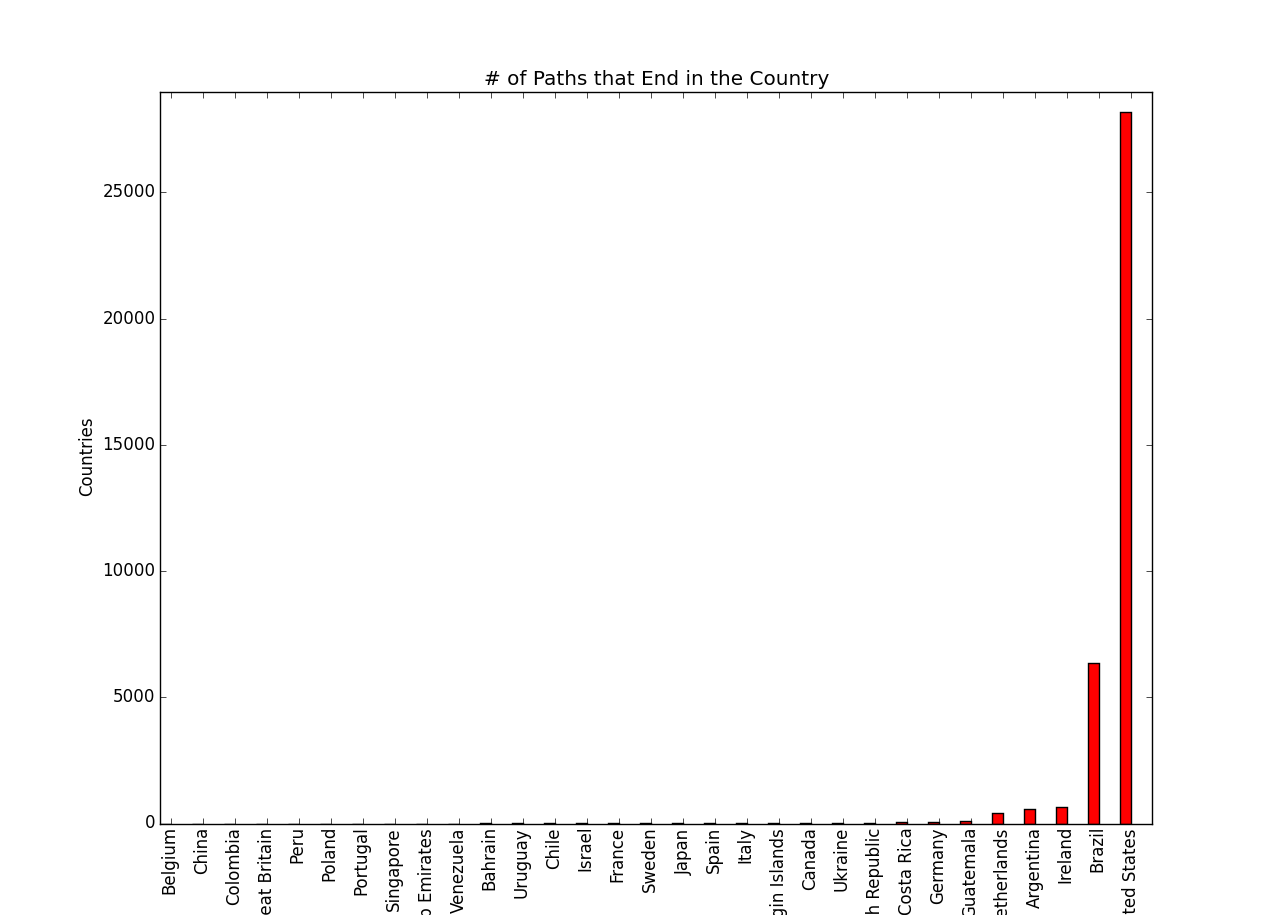
\includegraphics[width=.5\textwidth]{host_graph}
\caption{The number of paths that end in a country.}
\label{fig:host}
\end{figure}

\begin{figure}
\centering
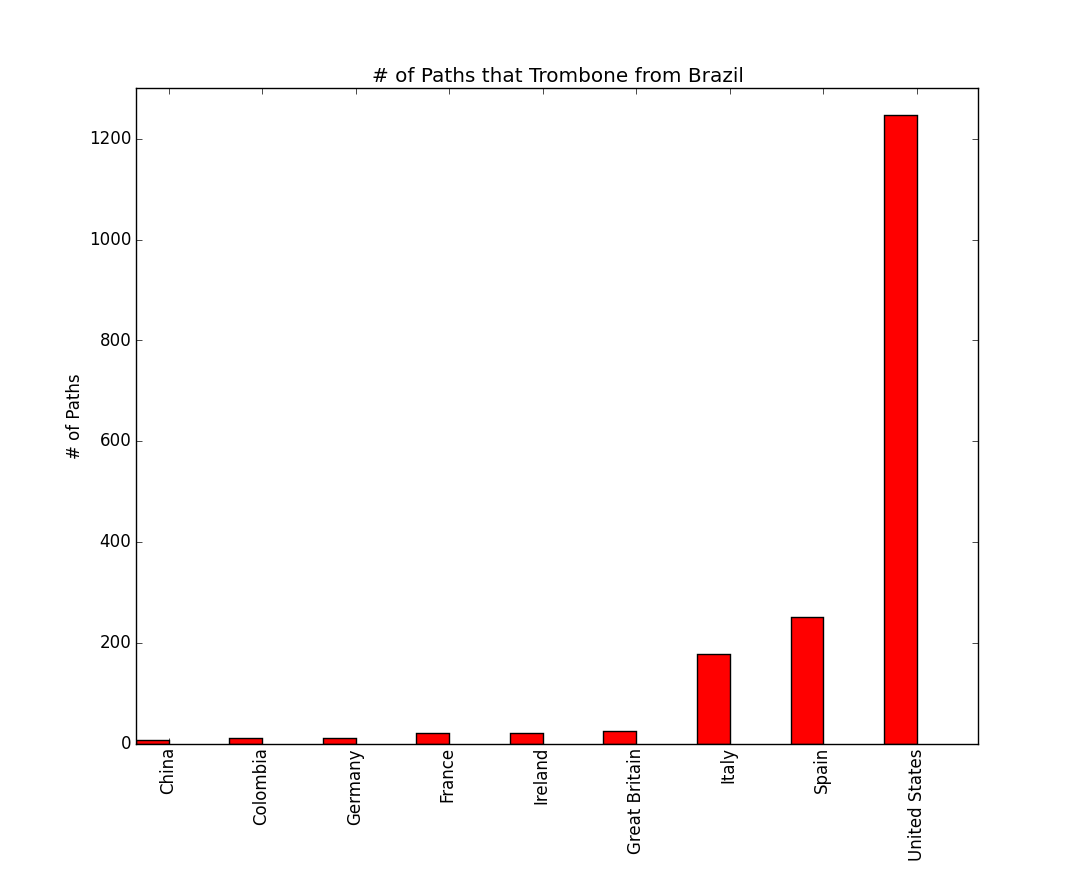
\includegraphics[width=.5\textwidth]{trombone_graph}
\caption{The number of paths that start and end in Brazil, but pass through another country.}
\label{fig:trombone}
\end{figure}
